Masked diffusion samplers treat acceptance as commitment: once a position is accepted, its token is final.
This section measures what that costs a uniform diffusion model.
One theoretical advantage of diffusion language models over autoregressive is the ability to self correct via iterative refinement.
However, the widely used masked diffusion does not allow for self correction without an explicit renoising schedule or corrector head.
Here we show that (1): DiffusionGemma exhibits self correcting properties that are driven by the model itself, not the sampler; and (2): the self correcting behavior enables it to have a robust Pareto frontier. 
\paragraph{Setup}
We focus on the EB sampler, as it is the default sampler used in \citet{team2026diffusiongemma}.
Our goal is to determine if DiffusionGemma exhibits self-correcting behavior, and whether this is driven by the model or the sampler.
To do this, we measure the macro-average of LCB v6, Natural2Code, and GPQA Diamond.
We introduce two intervention axes to investigate these questions: whether accepted tokens are "frozen" as in masked diffusion, and whether rejected tokens are renoised per the original sampler.

\paragraph{Frozen EB Sampler}
To do this, we first introduce a ``freezing'' variant of the EB sampler, where positions that are accepted under the EB rule cannot be changed later on, similar to masked diffusion.
We refer to the unmodified Unified EB sampler as ``unconstrained'', as any position can be changed regardless of whether it was already accepted under the EB rule.

\paragraph{No Noise}
To determine whether the self-correction is driven by the sampler, we additionally introduce a version of the sampler that does not renoise the rejected positions as done in the original sampler. 
If there is no additional noise injection, then the model must be able to directly correct mistakes as opposed to relying on the noise to reset incorrect positions.
This can be thought of as an Euler sampler, as it is strictly interpolating between a uniform random sample and the final sample.

\paragraph{Ablation}
Both the no noise and frozen EB sampler are orthogonal directions of intervention. Thus we ablate over all four combinations and show the results in Figure \ref{fig:frozen-eb-frontier}.
For each possible combination, we do a sweep over various entropy bound values to examine how they are affected by more relaxed thresholds. 
For the unconstrained variants, we also track the empirical frequencies of each position being altered during the denoising trajectory after the initial acceptance under the EB rule.
We show these position volatility metrics in Figure~\ref{fig:wasted} (bottom row).

% \begin{figure}[t]
%     \centering
%     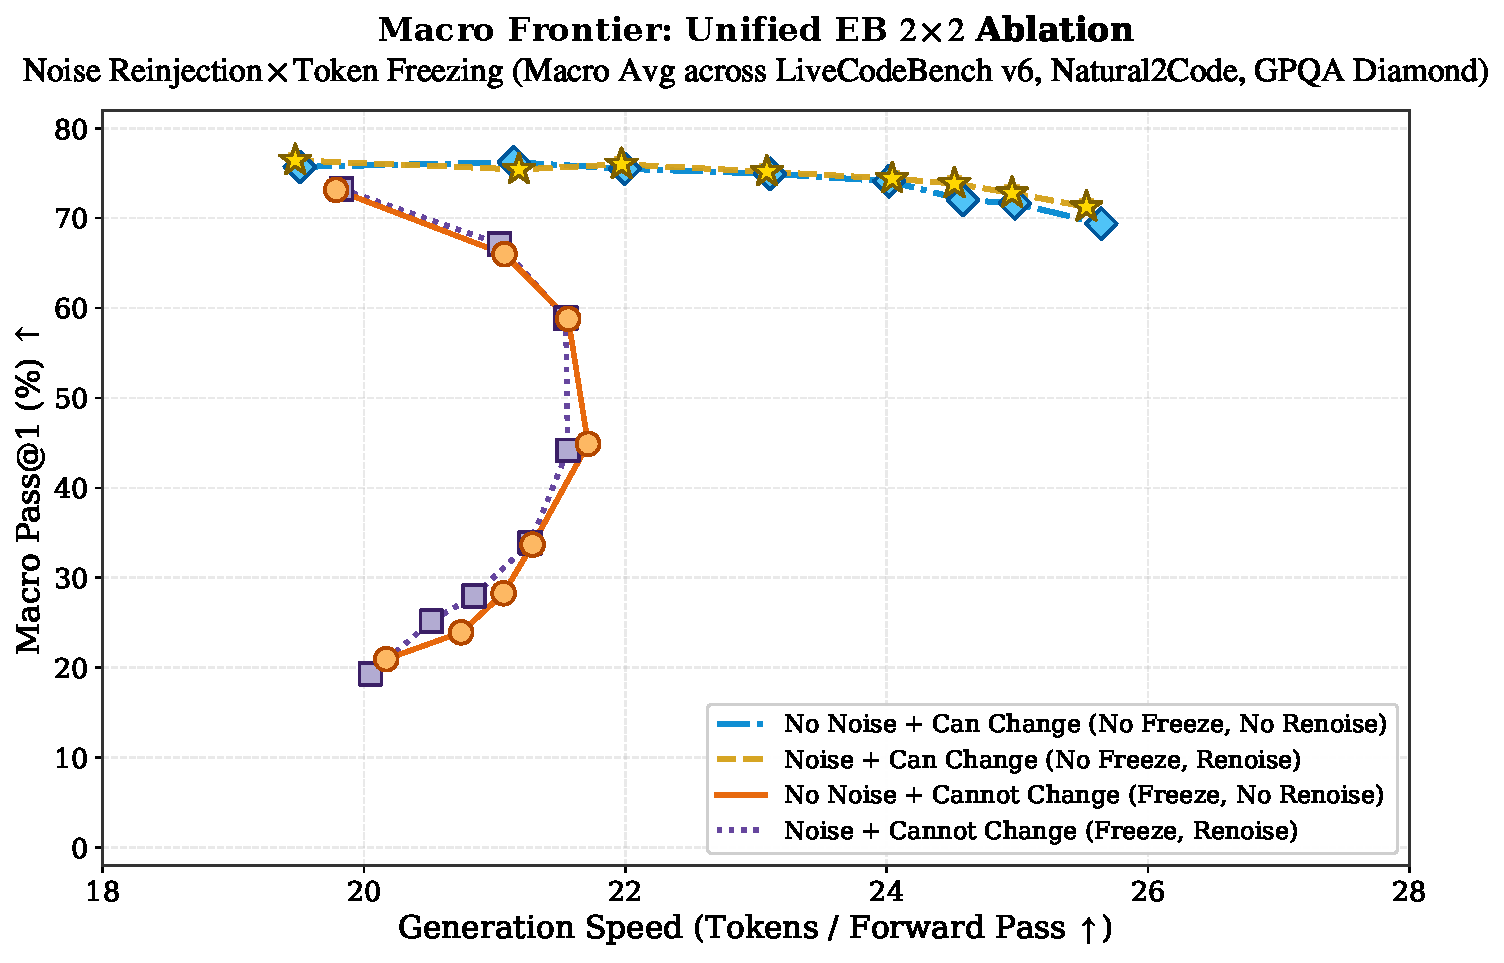
\includegraphics[width=1.0\linewidth]{images/fig_macro_frontier_unified_ablation_2x2.pdf}
%     \caption{We show the frontier for the modified DiffusionGemma EB sampler, where the entropy bound controls both the early stopping criterion and the commitment within a block. We observe that as the entropy bound grows, the sampler is able to increase throughput by sacrificing performance, producing a pareto frontier. The frozen variant of the EB sampler deteriorates performance much more rapidly than the base version, demonstrating that the flexibility of the uniform diffusion process contributes to the strong pareto frontier of DiffusionGemma.}
%     \label{fig:frozen-eb-frontier}
% \end{figure}


\paragraph{Results}
We observe that for each adaptive variant, the unconstrained sampler achieves a superior pareto frontier than the frozen sampler, and this gap increases with further relaxation of the thresholds.
At the loosest bound, the frozen variants fall to about 20\% macro Pass@1, while the unconstrained variants stay near 70\%.
Furthermore, the number of positions that change after initial acceptance increases with higher entropy thresholds, and is relatively unaffected by whether the sampler uses noise injection.
At the default bound of $0.1$, roughly 97\% to 99\% of accepted positions never change, so the default sampler behaves much like a frozen one; revisions become frequent only as the bound is relaxed.
This indicates that 1) the model does rely on self correction, as removing this deteriorates performance at relaxed thresholds; and 2) the self-correction is driven by the changes in the model's posterior as opposed to renoising, as removing noise does not alter post-acceptance behavior.

The design rule that follows is that acceptance must not be final: an accepted token should stay free to change until it is committed to the KV cache.
